\section{Оборудование}
\begin{figure}[ht!]
    \center{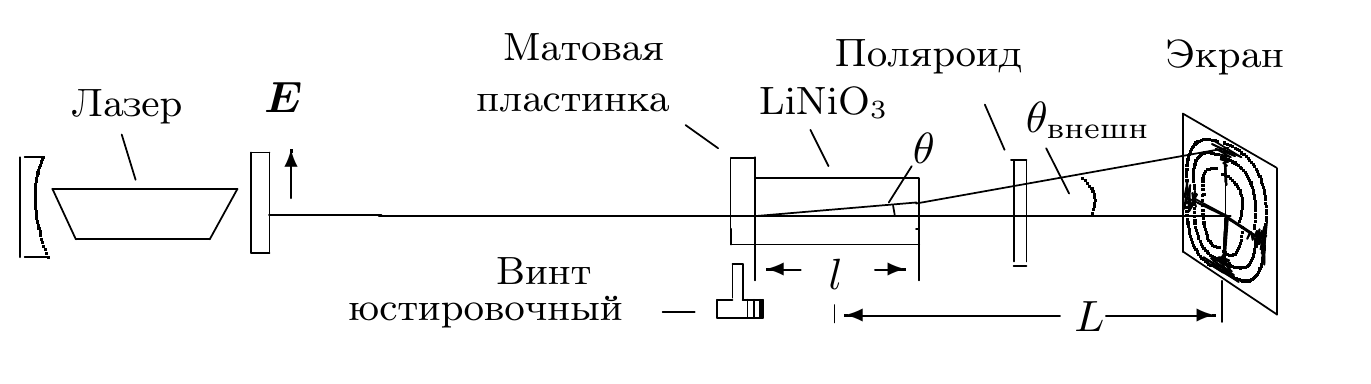
\includegraphics[width=0.8\linewidth]{../img/int.png}}
\end{figure}
\begin{figure}[ht!]
    \center{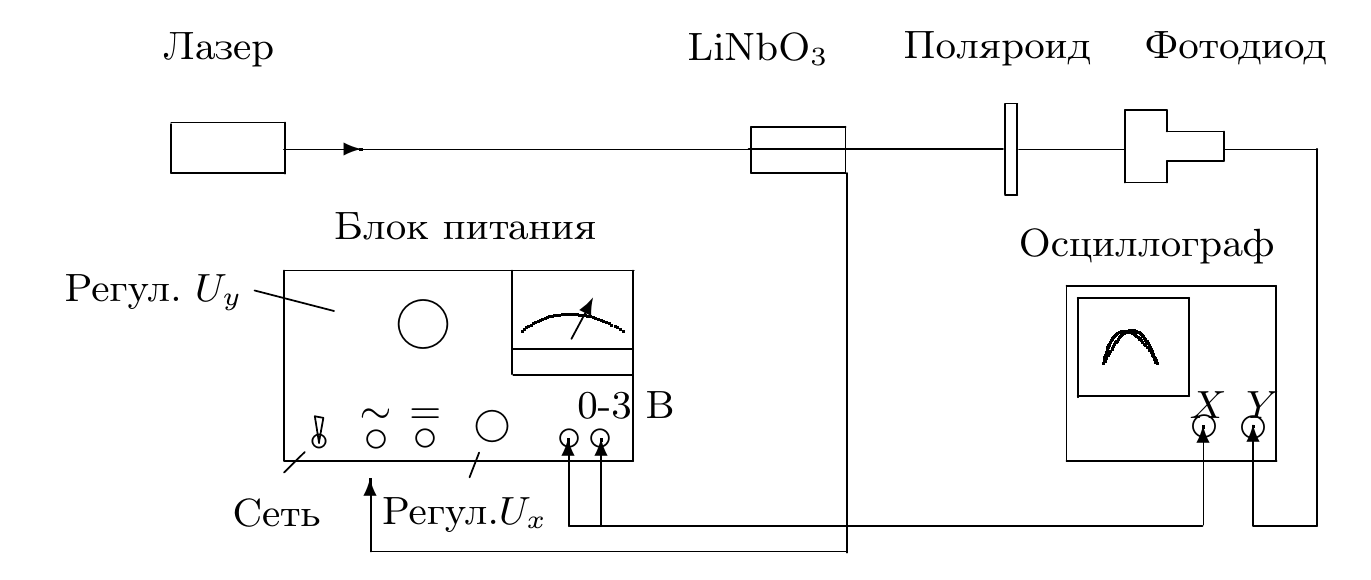
\includegraphics[width=0.8\linewidth]{../img/shit.png}}
\end{figure}

Схемы установок для наблюдения интерференции и изучения двойного лучепреломления в электрическом поле приведены на рисунках.

 Свет гелий-неонового лазера, поляризованный в вертикальной плоскости, проходя сквозь матовую пластинку, рассеивается и падает на двоякопреломляющий кристалл под различными углами. Кристалл ниобата лития с размерами $3 \times 3 \times 26\;\text{мм}$ вырезан вдоль оптической оси $z$. На экране, расположенном за скрещенным поляроидом, видна интерференционная картина.

 Для $\lambda = 0{,}63\;\text{мкм}$ в ниобате лития $n_{o} = 2{,}29$.

 Убрав рассеивающую пластинку и подавая на кристалл постоянное напряжение, можно величиной напряжения влиять на поляризацию луча, вышедшего из кристалла.

 Заменив экран фотодиодом и подав на кристалл переменное напряжение, можно исследовать поляризацию луча с помощью осциллографа.
